%----------------------------------------------------------------------------
%
%  $Description: General Research Plan Structure $
%
%  $Author: dloubach, with great contribution from rbonna $
%  $Release Date: December 20, 2016 $
%
%  O Projeto de Pesquisa deve demonstrar claramente os desafios científicos ou
%  técnicos a serem superados pela pesquisa proposta, os meios e métodos para
%  isso e a relevância dos resultados esperados para o avanço do conhecimento
%  na área.
%  Máximo 20 páginas.
%
%  The research project shall clearly demonstrate the scientific or techinical
%  chalenges to be overcame by the proposed research, as well as the ways and
%  methods to achieve so and moreover the expected results relevance to advance
%  the area knowledgement.
%  20 pages maximum.
%----------------------------------------------------------------------------
\documentclass[12pt, a4paper]{article}

% [portuguese|english], level=[undergrad | msc | phd]
\usepackage[portuguese, level=phd]{general-settings}

% [on | off]
\usepackage[on]{review-settings}


% title definitions
\newcommand{\researchTitle}{Análise de Escoamento em Superfícies Aerodinâmicas Utilizando Visão Computacional}
\newcommand{\researchTitleOtherLanguage}{Flow Analysis on Aerodynamic Surfaces Using Computer Vision}

% research level definitions
\newcommand{\studentName}{Cláudio Alexandre da Costa Dias}
\newcommand{\advisorName}{Luiz Alberto Vieira Dias}

% figures path
\usepackage{caption}
\graphicspath{{./figs/}}
\newcommand{\source}[1]{\vspace{-5pt} \caption*{ Fonte: {#1}} }

% space between lines
\linespread{1.3}

\begin{document}
% our title page
\makeourtitle

% contents
\tableofcontents

\newpage
\section*{Resumo}
Nos últimos anos, os métodos de aprendizado profundo demonstraram superar as técnicas anteriores de aprendizado de máquina de última geração em vários campos, sendo a visão computacional um dos casos mais proeminentes \cite{PMID:29487619}.

Neste trabalho, propõe-se a criação de um sensor inteligente que seja capaz de analisar imagens de uma superfície aerodinâmica e, em tempo real, identificar regiões desta superfície que apresentem determinadas características.

Para isto, será desenvolvido e treinado um modelo de redes neurais convolucionais (CNN) capaz de identificar padrões na visualização de escoamento em superfícies aerodinâmicas.

\textbf{Palavras chave --} aprendizado de máquina; redes neurais convolucionais; transferência de aprendizado; aerodinâmica; escoamento.


\newpage
\section*{\emph{Abstract}}
\begin{em}
Over the last years deep learning methods have been shown to outperform previous state-of-the-art machine learning techniques in several fields, with computer vision being one of the most prominent cases \cite{PMID:29487619}.

In this work, we propose the creation of an intelligent sensor that is able to analyze images of an aerodynamic surface and, in real time, identify regions of this surface that present certain characteristics.

For this, a model of convolutional neural networks (CNN) capable of identifying patterns in the visualization of flow on aerodynamic surfaces will be developed and trained.
\end{em}

\textit{\textbf{Keywords --} machine learning; convolutional neural networks; transfer learning; aerodynamics; flow}


\newpage
\section{\sectionI}
\label{sec:intro}
Na indústria aeronáutica, a necessidade de otimização da aerodinâmica é obviamente premente. Uma das técnicas frequentemente empregadas para esta otimização é a técnica de visualização de escoamento.

Várias técnicas de visualização de escoamento \cite{fisher1988flow} são atualmente empregadas como visualização por fumaça, emprego de materiais sensíveis à distribuição de pressão sobre superfícies aerodinâmicas, e utilização de \emph{tuffets} (tufos).

Na visualização do escoamento de superfícies aerodinâmicas em aeronaves em escala real (1:1) - em oposição à visualização em veículos em escala (empregados em túnel de vento, por exemplo) – dada a necessidade de embarcar-se a visualização durante o voo, a técnica dos tufos é preponderante sobre as demais.

Os tufos consistem em pequenos pedaços de lã, dispostos em \emph{grid}, colados sobre a superfície aerodinâmica de interesse. A orientação dos tufos em relação ao escoamento indica claramente as características deste escoamento.

\begin{figure} [ht]
    \centering
    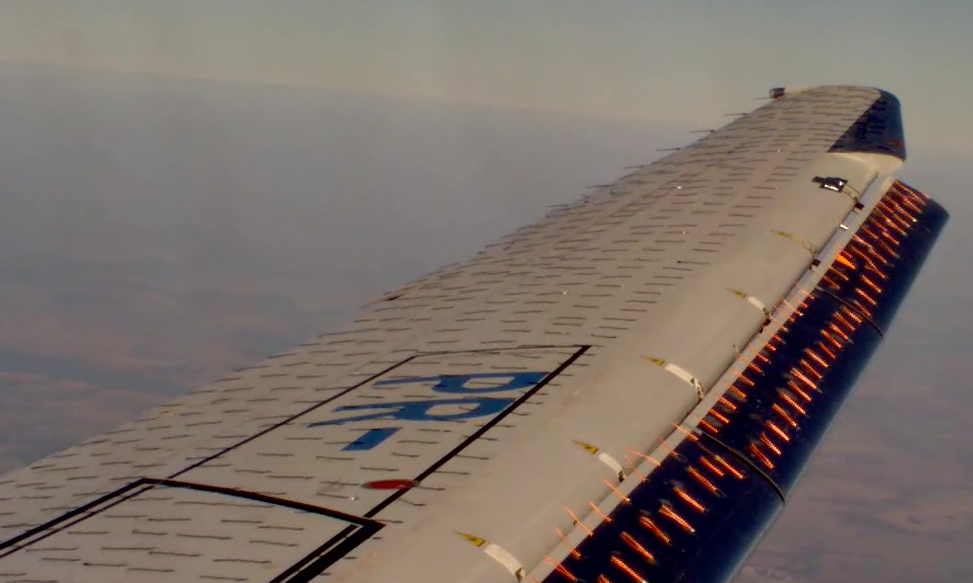
\includegraphics[width=0.95\textwidth]{tuffets.png}
    \caption{Tufos sobre a asa}
    \source{Embraer - Diretoria de Ensaios em Voo}
    \label{fig:tuffets}
\end{figure}

Na indústria aeronáutica, o emprego de câmeras (de diversas resoluções e velocidades) foi a evolução tecnológica mais recente e notável, uma vez que anteriormente havia necessidade de embarcar-se o aerodinamicista no veículo de testes para observação em “tempo real” do comportamento dos tufos durante o ensaio.

Com a adoção ampla do emprego de captura de imagens para visualização de escoamento, a análise dos resultados é atualmente feita por um ser humano treinado, durante reprodução das imagens gravadas a bordo. Tal técnica é frequentemente cansativa, extensa e maçante, dado o enorme volume de imagens normalmente adquiridas, além de bastante suscetível a erros (processo repetitivo) e altamente demandante.

Desta forma, o emprego de visão computacional na identificação de padrões nos tufos tem o potencial de substituir a atual técnica utilizada na análise.

\section{\sectionII}
\label{sec:rel-work}
% Esta seção deve apresentar, de forma breve, os principais trabalhos relacionados aos conceitos fundamentais da sua pesquisa.

% Busque dar uma visão ampla de trabalhos básicos fundamentais e também trabalhos mais recentes.
Wang \cite{Wang2003} disse que representar as emoções e consciência humanas ainda estavam no reino da ficção científica. Mas, muito mais importante, nos lembrou que as redes neurais são aproximadores universais de funções e deu alguns exemplos de redes neurais para previsão de séries temporais.

Atualmente, as redes neurais convolucionais fornecem uma boa base para a construção de um bom modelo de reconhecimento de padrões. Neste contexto, \cite{arxiv.1403.6382} apresenta resultados que sugerem fortemente que as \emph{features} obtidas a partir de aprendizado profundo com redes convolucionais devam ser o principal candidato na maioria das tarefas de reconhecimento visual.

Muitos modelos têm sido disponibilizados, e têm sido bastante utilizados em tarefas de reconhecimento diferentes daquelas para os quais eles foram treinados. Esta técnica de transferência de aprendizado vem sendo largamente usada para criar novos modelos que se utilizam do conhecimento obtido pelos modelos originais. \cite{arxiv.1411.1792} quantificam generalidade versus especificidade dos neurônios em cada nível da rede e apresentam resultados que indicam transferir o aprendizado de \emph{features}, mesmo de tarefas bem diferentes, pode ser melhor do que usar \emph{features} aleatórias.


\section{\sectionIII}
\label{sec:goal}
Criar de um sensor inteligente que seja capaz de analisar imagens de uma superfície aerodinâmica e, em tempo real, identificar regiões desta superfície que apresentem determinadas características.

Para isto, será desenvolvido e treinado um modelo de redes neurais convolucionais (CNN) capaz de identificar padrões na visualização de escoamento em superfícies aerodinâmicas.

\section{\sectionIV}
\label{sec:res-scope}
Este trabalho de pesquisa contém os seguintes tópicos:

\begin{itemize}
    \item Estudar e definir as características do escoamento numa superfície aerodinâmica;
    \item Estudar os tópicos pertinentes a este trabalho: aprendizado de máquina, redes neurais convolucionais, e  transferência de aprendizado;
    \item Definir e classificar imagens de voos anteriores que serão utilizadas como bases de treinamento e teste para o modelo;
    \item Criar e treinar um modelo que classifique as imagens dos tufos de acordo com características pré-definidas;
    \item Testar, e validar o modelo em laboratório utilizando vídeos de voos anteriores; e
    \item Testar, e validar o modelo durante um ensaio.
\end{itemize}

\section{\sectionV}
\label{sec:schedule}

\begin{enumerate}[A.]
    \item Cursar disciplinas e realizar treinamentos pertinentes;
    \item Revisão da literatura;
    \item Estudar escoamento em superfícies aerodinâmicas;
    \item Estudar aprendizado de máquina, redes neurais convolucionais, e  transferência de aprendizado;
    \item Desenvolver modelo de redes neurais convolucionais;
    \item Testar, e validar o modelo em laboratório; e
    \item Testar, e validar o modelo durante um ensaio.
\end{enumerate}

\begin{table}[ht]
    \centering
    \caption{Cronograma trimestral de atividades
    \label{tab:cronograma}}
    \begin{tabular}
        {|c||c|c|c|c||c|c|c|c||c|c|c|c||c|c|c|c||c|c|c|c|} \hline
        & \multicolumn{4}{|c||}{2020}
        & \multicolumn{4}{|c||}{2021}
        & \multicolumn{4}{|c||}{2022}
        & \multicolumn{4}{|c||}{2023}
        & \multicolumn{4}{|c|}{2024} \\ \hline \hline
        Trimestre & 1 & 2 & 3 & 4 & 1 & 2 & 3 & 4 & 1 & 2 & 3 & 4 & 1 & 2 & 3 & 4 & 1 & 2 & 3 & 4 \\ \hline \hline
        A & x & x & x & x & x & x & x & & & & & & & & & & & & & \\ \hline
        B & & & & & & & & x & x & & & & \ck & & \ck & & & & & \\ \hline
        C & & & & & & & & & & & x & \ck & & & & & & & & \\ \hline
        D & & & & x & x & x & x & x & x & x & x & \ck & \ck & \ck & & & & & & \\ \hline
        E & & & & & & & & & x & x & x & \ck & \ck & \ck & \ck & \ck & & & & \\ \hline
        F & & & & & & & & & & x & x & \ck & \ck & \ck & \ck & \ck & \ck & & & \\ \hline
        G & & & & & & & & & & & & & & & & & \ck & \ck & & \\ \hline
    \end{tabular}
\end{table}

Onde: \ck~ a fazer; x  concluída.

\section{\sectionVI}
\label{sec:parts-methods}
Que materiais (placas de hardware, kits de desenvolvimento, itens de medição) são necessários para desenvolver sua pesquisa?
Quais os métodos que vc pretente utilizar para desenvolver sua pesquisa? Colocar este tipo de informação nesta seção.


\section{\sectionVII}
\label{sec:result-analysis}
Como verificar/analisar se o que vc produziu está correto? \textit{Benchmark} disponível na literatura, estudos comparativos, reprodução de pesquisas? Como garantir a corretude dos resultados. Como verificar quão bom está o seu trabalho em relação ao que já existe atualmente?


% references
\bibliographystyle{ieeetr}
\bibliography{refs/references}

% todo list
% \listoftodos

\end{document}